\cotefile{156-6}
\scanpage{34}\mspage{33}

\uline{At$^{*}$2} Si $\Phi,\Psi\in{\unsure{\mathcal{F}|\mathscr{F}}}_M$, et $A\in\Phi\cap\Psi$, alors
$\Phi_A=\deleted{\unsure{\Phi}}\Psi_A$; i.e. la multistrate définie par $A$, soit dans
$\deleted{\unsure{\in\Phi}}\Phi$, soit dans $\Psi$, est \unsure{le|la} $=$.
% slanted
\margin{At$^{*}$1 et At$^{*}$2 impliquent \unsure{déjà} C\,1, C\,2 pour $\mathcal F$ $(\mathcal F_M,\leq\overset{\unsure{\mathrm{dfn}|\mathrm{déf}}}{=}\subset)$}

On l\deleted{'}a\deleted{ppellera} notera. $\deleted{\unsure{X|A}}\widetilde A$. ``Toute strate porte canoniquement une structure de multistrate'', indépendamment du \deleted{\unsure{le}} $\Phi\in\mathcal F_M$ dont c'est une strate.

\tikz[remember picture,overlay]\coordinate (msAtFour);
\uline{At$^{*}$\deleted{\unsure{3}}4} Si $\Phi,\Psi\in\mathcal F_M$ sont telles que $\forall\,A\in\Phi$, $B\in\Psi$, $\deleted{\unsure{\Phi_A\cup}}$ on ait $\Phi_A\cup\Psi_B\in\mathcal F_M$,
\margin{\uline{NB} il ne suffit \uline{pas} que $\Phi_A,\Psi_B$ soient compatibles \unsure{comme} figures ensemblistes!}
alors $\Phi\cup\deleted{\unsure{\Phi}}\Psi\in\mathcal F_M$.

\uline{At$^{*}$\deleted{\unsure{4}}5} L'ensemble $\deleted{\unsure{\mathcal{F}}}M^{*}$ de toutes les \deleted{\unsure{multi|mult}}strates \inserted{$A$} de \deleted{toutes} les $\Phi\in\mathcal F_M$ est une \unsure{figure} dans $M$ de support $M$. De plus,
$x,y\in M$, $x\ne y$, existe $A\in M^{*}$ telle que $x\in A$, $y\notin A$ ou $y\in A$, $x\notin A$.
($M^{*}$ ``sépare les points'' de $M$).
% slanted
\margin{i.e. tout $x\in M$ est contenu dans une strate \unsure{minimale|minim.}, les strates séparent les points, et \deleted{\unsure{pour}} \deleted{\unsure{une}} les \deleted{\unsure{strates}} strates \unsure{n'est|n'ont|ne sont} pas \unsure{réunion|réunions} des strates strictement \deleted{\unsure{plus}} contenues dans elles, (pour $\subset$)}
% The long arrow leads from the bracket at At*3 to the space just above At*4.

\tikz[remember picture,overlay]\coordinate (msAtThree);
\uline{At$^{*}$3} Soient $A,B$ deux strates relatives à $\mathcal F_M$ (i.e. des strates de $\Phi,\Psi\in\mathcal F_M$), telles que $A\subset B$, alors $\widetilde A\ll\widetilde B$\tikz[remember picture,overlay]\coordinate (msAtEnd);
\figure{\tikz[remember picture,overlay]{
  \draw ([xshift=7pt,yshift=8pt]msAtThree) .. controls +(-14pt,1pt) and +(-4pt,5pt) .. ([xshift=-5pt]msAtThree)
        .. controls +(-8pt,-7pt) and +(-13pt,0pt) .. ([xshift=7pt,yshift=-3pt]msAtThree |- msAtEnd);
  \draw[->] ([xshift=-5pt]msAtThree) .. controls +(-26pt,12pt) and +(-16pt,-12pt) .. ([yshift=8pt]msAtFour);
}}
% margin note written sideways
\margin{NB On \unsure{pourrait|p. maintenant} bloquer At$^{*}$2 et At$^{*}$3 en un seul : $\Phi,\Psi\in\mathcal F_M$, deux $A\in\Phi$, $B\in\Psi$, $A\subset B$ $\Longrightarrow\Phi_A\ll\Psi_B$. \uline{Cor.} Si $A=B$, $\Phi_A=\Psi_{\unsure{A|B}}$ d'où $A\mapsto\widetilde A$\,\ldots}

J'espère que je n'ai pas oublié d'axiomes!
\scanpage{35}\mspage{34}

\uline{20 juin} Comme
\[
\mathrm{Fig}(M)\longrightarrow\mathrm{Fig}(L)
\]
induit par l'application
\[
L\longrightarrow M
\]
est croissante pour $\leq$ et $\ll$, il s'ensuit que l'application
\[
\begin{aligned}
{\unsure{\mathcal F|\mathscr F}}&\longrightarrow\mathrm{Fig}(L) & F&\longrightarrow\unsure{\mathrm{Mulomb}|\mathrm{mulomb}}(F)\\
&&&(\uline{\text{petite}}\ \text{multiombre})
\end{aligned}
\]
est également croissante pour $\leq$ et $\ll$, et \unsure{commute} aux $\mathrm{Sup}$ pour $\leq$, et à $\mathrm{Inf}$ pour $\leq$. Mais elle n'est plus \unsure{néc|néc.} injective.
\margin{[\unsure{transforme} sous-figure en sous-figure.]}

\uline{Exemple 1}\quad \deleted{\unsure{a|1}}A) Soit $\deleted{X}E$ espace topologique, $\deleted{\unsure{A|M}}$
$\mathcal F$ l'ensemble des \deleted{figures ensemblistes} \deleted{paires} triples
\[
F=(X,\deleted{\unsure{\sigma}}\Sigma,\unsure{F|\Phi})
\]
où
\[
\begin{aligned}
&X\ \text{est une partie fermée de } E\\
&\Sigma\ \text{est une structure \unsure{lin.|liss.} par morceaux (disons, ou}\\
&\qquad\text{``\unsure{modérée}'' pour une théorie donnée) sur } X\\
&\Phi\ \text{est une figure ens. sur } X,\ \text{de support }X,\\
&\qquad\text{dont les strates sont des sous-ens. fermés}\\
&\qquad\text{lin. par morceaux.}
\end{aligned}
\]
\[
\begin{aligned}
(X',\Sigma',\Phi') &\leq (X^{\deleted{\unsure{\prime}}},\Sigma^{\deleted{\unsure{\prime}}},\Phi^{\deleted{\unsure{\prime}}})
\overset{\mathrm{dfn}}{\Longleftrightarrow}
\left\{\begin{aligned}
&\text{a) }X'\subset X\unsure{,|{}_{s}},\ \text{sous-espace lin.}\\
&\hspace{4em}\text{par morceaux pour }\Sigma\\
&\text{b) }\deleted{\unsure{\Sigma'} }\;\Sigma'\ \text{induite par }\Sigma\\
&\text{c) }\Phi'\leq\Phi
\end{aligned}\right.\\
(X',\Sigma',\Phi') &\ll (X,\Sigma,\Phi)
\overset{\mathrm{dfn}}{\Longleftrightarrow}
\left\{\begin{aligned}
&\text{a) et b) comme dessus}\\
&\text{c) }\Phi'\ll\Phi
\end{aligned}\right.
\end{aligned}
\]
On vérifie les axiomes. \unsure{L'ens.|D'ail.} $L$ s'identifie à $\deleted{X}E$, et l'application \unsure{en} $\mathcal F\longrightarrow\mathrm{Fig}(\deleted{\unsure{E}}L)=\mathrm{Fig}(E)$ est l'application $F\deleted{\mapsto}=(X,\Sigma,\Phi)\longmapsto\Phi$. Elle n'est visiblement pas injective en \unsure{générale|général|généralité} (p. ex. si $\deleted{\unsure{X}}E$ contient partie hom. à $[0,1]$).

B) \uline{Variante}\quad $M={}$ ens des \deleted{\unsure{parties de}} \inserted{couples} $X=(\deleted{X}A,\sigma)$ avec :
\[
\left\{\begin{aligned}
&\deleted{X}A\ \text{partie \deleted{\unsure{finie fermée|fermée|finie}} de }\deleted{X}E\\
&\sigma\ \text{une structure de \uline{simplexe affine} sur }\deleted{X}A\\
&\quad\text{d'où figure ensembliste }\Phi_\sigma\ \text{\unsure{sur|dans} }|\Phi_\sigma|=\deleted{X}A\\
&\quad\text{\unsure{son|de} support. l'inclusion }\deleted{X}A\subset E\ \text{continue.}
\end{aligned}\right.
\]
\scanpage{36}\mspage{35}

On pose
\[
\begin{aligned}
(\deleted{X}A',\sigma')\leq(\deleted{X}A,\sigma)&\overset{\mathrm{dfn}}{\Longleftrightarrow}
(\deleted{X}A',\sigma')\ \text{sous-simplexe \inserted{de $(A,\sigma)$} (face)}\\
(\deleted{X}A',\sigma')\ll(\deleted{X}A,\sigma)&\overset{\mathrm{dfn}}{\Longleftrightarrow}
\overset{\text{\inserted{de $(\deleted{X}A,\sigma)$}}}{\Phi_{\sigma'}\ll\Phi_{\sigma\deleted{\unsure{\prime}}}}\\
(\deleted{X}A,\sigma)\mathrel{\tikz[baseline=-.55ex,x=.85em,y=.70em]{\draw[line cap=round,line join=round] (0,1) .. controls (.22,.77) and (.86,.67) .. (.93,.61) .. controls (.82,.32) and (.28,.16) .. (.10,0); \draw[line cap=round,line join=round] (.98,1) .. controls (.77,.82) and (.43,.50) .. (.26,.37) .. controls (.43,.32) and (.72,.18) .. (.97,.04);}}(\deleted{X}A',\sigma')&\Longleftrightarrow
\deleted{X}A\cap\deleted{X}A'\ \text{est \inserted{vide ou} une face commune}\\
&\qquad\text{de }(X,\sigma)\text{ et }(X',\sigma')
\end{aligned}
\]

$\unsure{\mathcal F|\mathscr F}={}$ ens des parties finies (p. ex) de $M$, fermées pour $\leq$, et formées de simplexes $(A,\sigma)$ deux à deux compatibles

(\uline{NB} au lieu de ``finies'', on pourrait prendre aussi ``localement finies'')

Ici encore, $L\simeq E$, et ici
\[
M\longrightarrow\mathrm{Mulstrat}(L)\subset\mathrm{Fig}(L)
\]
n'est en général pas injectif (\unsure{par} p. ex. si $\deleted{X}E$ contient une partie homéomorphe \unsure{à} $[0,1]$!)

\uline{Exemple 2}\quad Considérons un ``pseudodisque'' $\deleted{\unsure{\partial B}\unsure{\supset|\to}B.}$ \deleted{Alors une} $(B,\partial B,\ldots)$ dans esp. top. $\deleted{X}E$.
Alors, \deleted{\unsure{la donnée (dans}} pour une définition convenable de l'ens des $\deleted{\unsure{F}}\mathcal F$ de (pseudo)-figures dans $E$, impliquant le type \deleted{topologique} \inserted{combinatoire} de
\figure{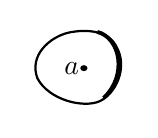
\begin{tikzpicture}[x=1cm,y=1cm]
\draw[line width=.8pt] (.03,.05) .. controls (-.08,.34) and (.18,.57) .. (.42,.63) .. controls (.65,.68) and (.94,.66) .. (1.04,.44) .. controls (1.18,.18) and (1.02,-.15) .. (.82,-.24) .. controls (.62,-.33) and (.18,-.23) .. (.03,.05) -- cycle;
\draw[line width=1.4pt] (.79,.64) .. controls (1.08,.57) and (1.18,.09) .. (.87,-.20);
\fill (.62,.18) ellipse (.046 and .038);
\node[left,inner sep=.7pt] at (.59,.18) {$a$};
\end{tikzpicture}}
(disque avec pt marqué) une figure de ce type, correspondant à $(B,\partial B)$, n'est pas \unsure{connue} par la seule connaissance de la partie (contractile etc) $\unsure{a|\bullet}$ de $B\setminus\partial B$ correspondant au ``centre'' du disque, mais il faut de plus se donner une ``structure de \unsure{reliement}'' de $a$ au bord\,\unsure{.....}.

Ceci étant, il est \inserted{sans doute} illusoire d'espérer que
\[
\begin{aligned}
&\deleted{\unsure{\mathcal F}\,\unsure{\mathrm{Mul}}\,\mathrm{mulomb}(F^{\unsure{\prime}})}\\
&\mathrm{mulomb}(F)\leq\mathrm{mulomb}(F')\Longrightarrow F\leq F'\\
&\mathrm{mulomb}(F)\ll\unsure{\mathrm{mulom}|\mathrm{mulomb}}(F')\Longrightarrow F\ll F',
\end{aligned}
\]
\scanpage{37}\mspage{36}

et en fait, le contraire est vrai dans les \inserted{\unsure{2|c$^{\mathrm t}$}} exemples 1. A) et B).

\uline{Définition}\quad On dit que $\unsure{\mathcal F|\mathscr F}$ est un \uline{atelier ensembliste} si pour $F,G\in\mathcal F$, on a
\[
\begin{aligned}
&\text{a) }\mathcal F\longrightarrow\mathrm{Fig}(L)\quad\text{injectif}\\
&\text{b) }\mathrm{mulomb}\,F\leq\mathrm{mulomb}\,G\Longrightarrow F\leq G\\
&\text{c) }\mathrm{mulomb}\,F\ll\mathrm{mulomb}\,G\Longrightarrow F\ll G\\
&\deleted{\unsure{\mathrm{d)}}}\ \unsure{\mathrm{d)}}\,\mathrm{mulomb}\,F\mathrel{\tikz[baseline=-.55ex,x=.85em,y=.70em]{\draw[line cap=round,line join=round] (0,1) .. controls (.22,.77) and (.86,.67) .. (.93,.61) .. controls (.82,.32) and (.28,.16) .. (.10,0); \draw[line cap=round,line join=round] (.98,1) .. controls (.77,.82) and (.43,.50) .. (.26,.37) .. controls (.43,.32) and (.72,.18) .. (.97,.04);}}\mathrm{mulomb}\,G\Longrightarrow F\mathrel{\tikz[baseline=-.55ex,x=.85em,y=.70em]{\draw[line cap=round,line join=round] (0,1) .. controls (.22,.77) and (.86,.67) .. (.93,.61) .. controls (.82,.32) and (.28,.16) .. (.10,0); \draw[line cap=round,line join=round] (.98,1) .. controls (.77,.82) and (.43,.50) .. (.26,.37) .. controls (.43,.32) and (.72,.18) .. (.97,.04);}}G\deleted{\unsure{\mathcal F}}\\
&\deleted{\mathrm{mulomb}(F)\ \text{élémentaire}\ \Longleftrightarrow}
\end{aligned}
\]
% slanted
\margin{De \unsure{toutes façons|toute façon}, un axiome ultérieur, imposé pour \uline{\unsure{tout}} atelier, \unsure{indiquerait|indiquera} que \deleted{\unsure{pour}} $\mathrm{mulomb}(F)$ élémentaire $\Longleftrightarrow F$ élémentaire}

(NB peut-être qu'on sera amené encore à renforcer ces conditions), de telle sorte que
\[
\mathcal F\longrightarrow\mathrm{Fig}(L)
\]
identifie $\mathcal F$, avec les structures $\leq,\ll,\mathrel{\tikz[baseline=-.55ex,x=.85em,y=.70em]{\draw[line cap=round,line join=round] (0,1) .. controls (.22,.77) and (.86,.67) .. (.93,.61) .. controls (.82,.32) and (.28,.16) .. (.10,0); \draw[line cap=round,line join=round] (.98,1) .. controls (.77,.82) and (.43,.50) .. (.26,.37) .. controls (.43,.32) and (.72,.18) .. (.97,.04);}}$, à un \deleted{sous-ensemble} ``sous-atelier'' de $\mathrm{Fig}(L)$.

Je voudrais préciser ce point, \deleted{en termes de} \inserted{D'abord}

\uline{Définition}\quad Soient $(\mathcal F,\leq,\ll)$ et $(\mathcal F',\leq,\ll)$ deux ateliers, $f=\unsure{f_{\mathrm{fig}}^{\prime}|f_{\mathrm{fig}}}\colon\mathcal F\longrightarrow\mathcal F'$ une application. On dit que $f$ est un \uline{morphisme d'ateliers} si

a) $f$ croissante pour $\leq$ et $\ll$

b) \deleted{$f$ transforme \unsure{sous}} $f$ commute aux $\mathrm{Sup}$ pour $\leq$ \inserted{(\unsure{d'où} $\varnothing_{\mathcal F}\mapsto\varnothing_{\mathcal F'}$)}, et aux $\mathrm{Inf}$ \inserted{\deleted{\unsure{major|non}} des familles \unsure{majorées|n.v. paires}} pour $\leq$

\deleted{\unsure{c)} $f$ transforme figures élémentaires} \deleted{\unsure{Cela|(cela} revient au $=$ que de se donner} 

% margin note written sideways
\margin{En fait, si $F'=f(F)$ alors $\mathcal F_{\leq F}\simeq{\unsure{\mathcal P|\mathfrak P}}_{\mathrm{fermés}}(\widetilde F)$ $\mathcal F'_{\leq F'}\simeq\mathcal P_{\unsure{\mathrm{fermé}|\mathrm{fermés}}}(\widetilde F')$, et l'application $(*)$\tikz[remember picture,overlay]\coordinate (ms37UpperNote); \unsure{semble} être \unsure{induite|induit} \unsure{tjs|tjrs} par $\widetilde F'\unsure{\rule[.5ex]{1.35em}{.6pt}|\longrightarrow}\widetilde F$ \uline{croissante} \inserted{i.e. continue} et $=$ telle que \unsure{tt|le} \unsure{fermé|suppt} de $\widetilde F'$ soit image inv. de un \unsure{fermé} de $\widetilde F$\,\ldots}
% slanted
\margin{\tikz[remember picture,overlay]\coordinate (ms37PairOne);\uline{NB} a) Dans tous les exemples que j'ai vus, $\deleted{\unsure{A|\forall}}\forall\,F\in\mathcal F$, l'application induite par $f$ $(*)\tikz[remember picture,overlay]\coordinate (ms37LowerNote);\ \mathcal F_{\leq F}\longrightarrow\mathcal F'_{\leq f(F)}$ est \uline{surjective}. \tikz[remember picture,overlay]\coordinate (ms37PairTwo);b) Dans la plupart des cas (``cas ensembliste'', \unsure{notamment|notam$^{\mathrm t}$}) $f$ est croissante pour $\unsure{\preceq|\leq}$ également\,\ldots}
\figure{\tikz[remember picture,overlay]{
  \draw[->] ([xshift=-2pt,yshift=1pt]ms37LowerNote) .. controls +(13pt,14pt) and +(4pt,-12pt) .. ([xshift=-2pt,yshift=-1pt]ms37UpperNote);
  \draw ([xshift=-3pt,yshift=5pt]ms37PairOne) -- ([xshift=-3pt,yshift=-6pt]ms37PairOne);
  \draw ([xshift=-4.5pt,yshift=5pt]ms37PairOne) -- ([xshift=-4.5pt,yshift=-6pt]ms37PairOne);
  \draw ([xshift=-3pt,yshift=5pt]ms37PairTwo) -- ([xshift=-3pt,yshift=-7pt]ms37PairTwo);
  \draw ([xshift=-4.5pt,yshift=5pt]ms37PairTwo) -- ([xshift=-4.5pt,yshift=-7pt]ms37PairTwo);
}}

$\deleted{\unsure{f_{\mathrm{str}}}\colon M\longrightarrow M'}$
On dit \deleted{telle que} que $f$ est ``compatible aux strates'' si $f$ satisfait \deleted{\unsure{a)} $f$ croissante pour} en plus

c) $f$ transforme multistrates \inserted{(i.e. fig. él.)} en multistrates \inserted{(fig. él.)}

Alors la donnée d'une telle $f$ équivaut à celle de
\[
\unsure{f_{\mathrm{strat}}|f_{\mathrm{str.t}}}\colon M\unsure{\rule[.5ex]{1.65em}{.65pt}|\longrightarrow}M'
\]
\scanpage{38}\mspage{37}

satisfaisant

a) $f_{\unsure{\mathrm{str}|\mathrm{str.}}}$ croissante pour $\leq$ et $\ll$

b) $\deleted{\unsure{f_{\mathrm{str}}}}$ \deleted{\unsure{pour tout|pour toute}} $F\subset M$ provient d'une figure, $f_{\mathrm{str}}(F)$ est une figure

\margin{\tikz[baseline=(ms38NB.base)]{\node[inner sep=.5pt] (ms38NB) {\uline{NB}}; \draw ([xshift=2pt]ms38NB.north east) -- (ms38NB.north west) -- (ms38NB.south west) -- ([xshift=1pt]ms38NB.south east);} Pour que $f$ soit inj. il f et s que $f_{\mathrm{str}}$ le soit. Pour que ce soit un iso. avec un sous-atelier \deleted{strict}, il f. et s. que $f$ soit un plongement pour $\leq$ et $\ll$, et que l'image soit $\leq$-fermée.$^{*}$}
% slanted
\margin{Mais le sous-atelier n'est pas strict pour autant -- dire qu'il l'est \unsure{signifie} que toute partie de $f(M)\subset M'$ qui est une figure pour $\unsure{\mathcal F|\mathscr F}\mathstrut'$, en est déjà une pour $\mathcal F$}

On appelle \uline{sous-atelier} d'un atelier, une \deleted{\unsure{de}} partie $\mathcal F'$ de $\mathcal F$, telle que, munie des relations d'ordre $\underset{\mathcal F'}{\leq},\underset{\mathcal F}{\ll}$ induites par celles de $\mathcal F$, ce soit un atelier, et que $\mathcal F'\hookrightarrow\mathcal F$ soit un morphisme d'ateliers, i.e. que

$1^{\circ}$) Si $F_i\in\mathcal F'$ sont majorés \uline{dans} $\mathcal F'$, \inserted{pour $\leq$} alors
\[
\mathop{\mathrm{Sup}}\limits_{i\,(\mathcal F)}F_i\in\mathcal F'\qquad\text{(stabilité par Sup majorés)}
\]
$2^{\circ}$) Sous \deleted{\unsure{la}} les $=$ hypothèses, $\bigcap F_i\in\mathcal F'$

% slanted
\margin{Mais on ne suppose pas que, si $F,F'\in\mathcal F'$ et $F\vee F'$ existe dans $\mathcal F$ (i.e. $\{F,F'\}$ majorés dans $\mathcal F$) on ait $F\vee F'\in\mathcal F'$ i.e. $\{F,F'\}$ majoré dans $\mathcal F'$. Donc on ne suppose \deleted{pas} $\mathcal F'$ stable par sommes (quand elles \unsure{ne le sont|ne sont} majorées dans $\mathcal F'$) Le sous-atelier est dit (\uline{\unsure{spacieux}} ou \uline{strict}) s'il est stable pour Sup dans $\mathcal F$ (\unsure{pas néc.|pour néc.} majorés)}

\tikz[remember picture,overlay]\coordinate (msQuestionTop);
\unsure{Je} me demande s'il ne serait pas plus raisonnable, au lieu de $1^{\circ}$, et $2^{\circ}$, de poser

$\text{\textcircled{\scriptsize $*$}}$\quad \uline{Si} $F'\in\mathcal F'$, \deleted{et $F\in\mathcal F$ est tel que $F$} \inserted{\uline{alors \unsure{tte|toute} sous figure}} $F'$ \uline{est dans} $\mathcal F'$.

Il faut vérifier \inserted{seulement} que cette condition suffit à impliquer que $(\mathcal F',\underset{\mathcal F'}{\leq},\underset{\mathcal F'}{\ll})$ est bien un atelier\,\ldots\tikz[remember picture,overlay]\coordinate (msQuestionEnd);
\figure{\tikz[remember picture,overlay]{
  \draw ([yshift=6pt]msQuestionTop) -- ([xshift=-4pt,yshift=6pt]msQuestionTop)
    -- ([xshift=-4pt,yshift=-2pt]msQuestionTop |- msQuestionEnd) -- ([yshift=-2pt]msQuestionTop |- msQuestionEnd);
}}

Les sous-ateliers \inserted{stricts} correspondent aux sous ens. \inserted{$M'$} de $M$ fermés pour $\leq$, sans plus,
% slanted
\margin{En tous les cas, si $\mathcal F'$ est un sous-atelier de $\mathcal F$, $\mathcal F'\unsure{\rule[.5ex]{1.4em}{.55pt}|\longrightarrow}\mathcal F$ est \deleted{\unsure{un}} un morphisme strict et $M'$ s'identifie à l'ens des fig. él. dans $\mathcal F$. (et $M'=\mathcal F'\cap M$?)}

Donc, $\mathcal F$ est dit ensembliste, si l'application $\mathrm{mulomb}\colon\mathcal F\unsure{\rule[.5ex]{1.4em}{.55pt}|\longrightarrow}\mathrm{Fig}(L)$ le ``réalise'' comme sous-\unsure{atelier} de $\mathrm{Fig}\,L$ -- en fait, on aimerait que ce soit un sous-atelier \uline{strict}$^{*}$,
% slanted
\margin{$^{*}$ C'est donc une \unsure{condition} plus forte encore que dans la définition de la page précédente, où d) implique seulement la stabilité pour $F\vee G$, et pas pour les Sup quelconques.}
et on voudra \deleted{que} en particulier que $M$ se réalise comme un ens de figures élémentaires (ou multistrates ensemblistes) \uline{dans $L$}. Ainsi, dans la définition de la page précédente, il faudra \unsure{rajouter|se contenter|se pencher}
\scanpage{39}
\mspage{38}
des conditions : $\unsure{\mathcal F|\mathscr F}$ stable dans $\mathrm{Fig}(L)$ par passage à une sous-figure, et par $\mathrm{Sup}_{\leq}$ (\unsure{ces deux-ci donc|ces deux ci-dessus} renforcent d).

Je reprends ces définitions

% One long oblique cancellation runs from the left of Soit to the foot of the sheet.
\tikz[remember picture,overlay]\coordinate (ms39DefStart);
\deleted{\uline{Définition} \quad Soit $(\mathcal F,\deleted{\unsure{\sim|\leq}}\leq,\ll)$ un atelier At1--At7 (on verra pour les axiomes ultérieurs pour \unsure{la suite|$C$ ouverts|$\mathcal C$ ouverts}).}
% slanted
\margin{\uline{Non} vide équivaut à $\varnothing_{\mathcal F}\in\mathcal F'$}

\deleted{Un \uline{sous-atelier} est une \deleted{(non vide)} partie $\mathcal F'$ \inserted{\uline{non vide}} de $\mathcal F$, fermée pour $\leq$, (i.e. telle que \unsure{t|l}\deleted{\unsure{oute|te}} sous-figure d'une figure dans $\mathcal F'$ est dans $\mathcal F'$), \inserted{et stable par $\mathrm{Sup}$ majorés dans $\mathcal F'$} On dit que $\mathcal F'$ est \inserted{un sous-atelier} \uline{spacieux} s'il est \inserted{de plus} stable par $\mathrm{Sup}$ quelconques (sans les supposer majorés dans $\mathcal F'$).}\tikz[remember picture,overlay]\coordinate (ms39DefEnd);

\deleted{Ces notions \deleted{\unsure{sont abs|sont dé}} ne dépendent que de $\leq$. Mais on munira bien sur $\mathcal F'$ des \deleted{\unsure{la|le}} \uline{deux} relations $\leq,\ll$ induites.}

\tikz[remember picture,overlay]\coordinate (ms39Soit);
\deleted{Soit}
\[
\deleted{M'=\mathcal F'\cap M}
\]
\tikz[remember picture,overlay]\coordinate (ms39Strict);
\deleted{alors on voit que les objets de $M'$ sont les objets (strictement) irréductibles \inserted{(\unsure{cf.|v.} \unsure{Ch$^{\mathrm{re}}$|Ch.} \uline{IV}, p.\,\unsure{53|52})} de $\mathcal F'$ pour $\leq$\unsure{? |;|:}. En effet, si $\deleted{\unsure{X|x}}X\in\deleted{\unsure{M'|\mathcal F}}\mathcal F'$, \deleted{et si} \inserted{\deleted{\unsure{les|les m}}\unsure{comme|même} $\mathcal F'$ est \unsure{fermé|fermée}} \deleted{$X=\mathop{\mathrm{Sup}}\limits_i\unsure{F_i|A_i}$ dans,}}
\deleted{\deleted{on a aussi $X=\mathrm{Sup}\,\unsure{F_i|E_i}$ dans $\mathcal F$ (car $\mathcal F'$ est fermé dans $\mathcal F$)} \deleted{par hyp. donc $\exists i$ avec $X=F_i$, donc $X$ irr dans $\mathcal F'$} \deleted{Inversement, si $X\in\mathcal F'$ est irr} \unsure{--|.} dans $\mathcal F$, dans $\mathcal F$, les familles $\{F_i\}$ dans $\mathcal F'$, \inserted{majorées par $X$}, sont les $\unsure{=\mathrm s|\Longleftrightarrow\mathrm s}$. Comme $\mathcal F'$ \deleted{est stable par} \inserted{$\hookrightarrow\mathcal F$ commute aux} $\mathrm{Sup}$, dire que pour une telle famille, $X=\mathrm{Sup}\,F_i$ dans $\mathcal F'$, revient au $=$. \deleted{\unsure{O|P}}Dire que pour \unsure{ttes|toutes} telles familles, $\exists i$ avec $\unsure{X_i|X}=F$, est \unsure{itou|idem} pour $\mathcal F$ ou $\mathcal F'$.}

\figure{\tikz[remember picture,overlay]{
  \draw ([xshift=-4pt,yshift=-6pt]ms39DefStart) .. controls +(-1.5pt,0pt) and +(-1pt,1pt) .. ([xshift=-4pt,yshift=-2pt]ms39DefStart |- ms39DefEnd);
  \draw ([xshift=-4pt]ms39Soit) -- ([xshift=-4pt,yshift=-12pt]ms39Soit |- ms39Strict);
  \draw ([xshift=-5.6pt]ms39Soit) -- ([xshift=-5.6pt,yshift=-11pt]ms39Soit |- ms39Strict) -- ([xshift=-4pt,yshift=-12pt]ms39Soit |- ms39Strict);
}}
\deleted{\deleted{Il faudrait vérifier}}

\deleted{Dans le cas d'un \inserted{sous-}atelier spacieux, on récupère}
\scanpage{40}
\mspage{39}
% Three oblique strokes cancel the first definition and stop above the fresh Soit.
\deleted{\uline{Définition} \quad Soit $(\deleted{\unsure{I|\mathcal J}}\unsure{\mathcal F|\mathscr F},\leq)$ un ens ordonné \inserted{avec $\mathrm{Sup}$ majorés et plus petit élément $\varnothing_{\mathcal F}$}. Une partie fermée $\mathcal F'$ de $\mathcal F$ est dite \uline{ample} si $\mathcal F'$ \deleted{\unsure{est|$\ne\varnothing$}} est stable par $\mathrm{Sup}$. majorés \uline{dans} $\mathcal F'$, \inserted{et $\mathcal F'\ne\varnothing$ $(\Longleftrightarrow\varnothing_{\mathcal F}\in\mathcal F')$.} On dit qu'elle \unsure{est|\deleted{est}} est \uline{\unsure{spacieuse|spacieux}} si elle est \deleted{stable par} $=$ \deleted{\unsure{spa|sp}}stable par $\mathrm{Sup}$ majorés dans $\mathcal F$.}

Soit $(\mathcal F,\leq)$ un ens. ordonné \deleted{stable par} \inserted{avec} $\mathrm{Sup}$. majorés et plus petit \unsure{élément|élmt} $\varnothing_{\mathcal F}$\inserted{(i.e. \unsure{satisfais.|satisf.} à At1}.

Soit $\deleted{\unsure{F|\mathcal J}}\mathcal F'$ une partie \uline{fermée}. Alors donc $\mathcal F'$ \deleted{\unsure{lors|les}} est non vide sss $\varnothing_{\mathcal F}\in\mathcal F'$. D'autre part, si $(F_i)$ est une famille dans $\mathcal F'$ qui est majorée dans $\mathcal F'$ par $\deleted{\unsure{F|H}}G$, alors son sup dans $\mathcal F$, soit $F$, est $\leq G$, donc $\in\mathcal F'$, et c'est un sup dans $\mathcal F'$. Donc $\mathcal F'$ est stable par sup. majorés dans $\mathcal F'$\inserted{(il satisfait donc At 1)}, et $\mathcal F'\hookrightarrow\mathcal F$ commute à ces sup.

Soit $\deleted{\unsure{X|N}}M$ l'ens des éléments (\unsure{str$^{\mathrm{t}}$|str.}) irréductibles de $\mathcal F$, et
\[
M'=M\cap\mathcal F'.
\]
Alors : $M'$ est l'ens des objets (str.) irréd. de $\mathcal F'$. En d'autres termes, si $F\in\mathcal F'$, pour que $F$ soit irréd. dans $\mathcal F'$, il f et s qu'il le soit dans $\mathcal F$. C'est immédiat, en termes des définitions (les familles $(\deleted{\unsure{d|A}}F_i)$ d'objets \deleted{\unsure{de|du}} majorés par $F$, que ce soit ds $\mathcal F$ ou $\mathcal F'$, sont les $=\mathrm{s}$, et leurs $\mathrm{Sup}$ dans $\mathcal F$ ou $\mathcal F'$ \unsure{itou|idem}, donc celles pour lesquelles $F=\mathrm{Sup}\,F_i$ sont les $=\mathrm{s}$, et dire que pour
\scanpage{41}
\mspage{40}
telle famille, $\exists i$ t.q. $F_i=F$, est \inserted{donc} pareil dans $\unsure{\mathcal F|\mathscr F}$ et $\mathcal F'$. )

Supposons que $\mathcal F$ satisfasse At 2 :
\[
\begin{aligned}
\forall F\in\mathcal F,\ \text{on a}\qquad
 F&=\mathop{\mathrm{Sup}}\limits_{X\in\deleted{\unsure{F|\mathcal F}}\widetilde F\unsure{.|,}}X
 &\qquad \text{où}\quad \widetilde F&=\{X\in M\mid X\leq F\}\\
 &&&=\{X\in\mathcal F,\ X\triangleleft F\}.
\end{aligned}
\]
Alors $\mathcal F'$ y satisfait aussi, car si $F\in\mathcal F'$, $\widetilde F$ au sens de $\mathcal F$ ou de $\mathcal F'$ c'est pareil, et le sup dans $\mathcal F$ est un sup dans $\mathcal F'$.

\uline{Définition} \quad La partie fermée $\mathcal F'$ \deleted{\unsure{ou de|est de}} de $\mathcal F$ est dite \uline{spacieuse} si elle est stable par $\mathrm{Sup}$ quelconques (de familles majorées \uline{dans $\mathcal F$}).
% slanted
\margin{On dira qu'elle est \uline{finiment} \uline{spacieuse} si elle est stable par $\mathrm{Sup}$ finis.}
% slanted
\margin{\unsure{Remords|Remonde} : il vaut mieux réserver le mot ``spacieux'' à la notion la plus modeste des deux, et appeler l'autre ``infiniment spacieux'' ou ``très spacieux''.}

\uline{Exemple} \quad Soit $\mathcal F$ \inserted{$=\unsure{\mathcal P|\mathfrak P}(I)$} l'ens des parties d'un ens. $I$, \deleted{Alors $\mathcal F'$} avec la relation d'inclusion. Satisfait At 1, At 2, At 3, \deleted{\unsure{les|la}} $M=\{\{i\}\mid i\in I\}$ (avec \unsure{ordre|l'ordre} discret), \inserted{(si $I$ est fini)}
$\deleted{\unsure{\mathcal F|I}}$Se donner une $\mathcal F'$ \inserted{\deleted{fer\unsure{mée|mé}} \uline{\unsure{ample|sp}}} revient au $=$ que de se donner une structure de \deleted{\unsure{pr|s}} \deleted{\unsure{quelque|quels|quasi}} simpliciale sur \inserted{une partie $\unsure{I'|I}\deleted{\unsure{\subset|=}}=\mathcal F'\cap I$ de} $I$, du moins si $I$ est fini. (Sinon, c'est vrai à condition de se restreindre aux $\mathcal F'$ \unsure{formés|fermés} d'ens. finis \ldots).

Dire que $\mathcal F'$ est spacieux, signifie que \deleted{\unsure{tout|toute}} réunion de simplexes est une simplexe -- se donner un tel $\mathcal F'$, revient donc à se donner une partie $I'$ de $I$, \deleted{$\mathcal F'$ est} et $\deleted{\unsure{F|\mathcal J}}\mathcal F'=\mathcal P(I')$ -- c'est pas du \deleted{tout} pareil !
